

\chapter{Theory}
\label{chapter:theory}

\section{Protocol Attacks: TCP SYN Flooding}

TCP (Transmission Control Protocol) is one of the most common protocols within the transport layer, and one of the core of the Internet Protocol suite (IP). TCP provides reliable, ordered, error-checked of stream of packets between two hosts. In addition to these characteristics, TCP is a connection-oriented protocol, that is, before starting the exchange of information a prior connection between both parties is necessary. This process is known as TCP three-way handshake (Figure\ref{fig:TCPHandshake}).

\par

Suppose \textit{X} as a client that wants to carry out a friendly TCP connection with the server \textit{Y}. First of all, \textit{X} requests by sending a synchronize \textit{(SYN)} message to \textit{Y}. The server receives the request and responses by sending an acknowledge \textit{(SYN-ACK)} back to the client. Once the client receives the SYN-ACK, it responses with an ACK, an the connection is established. 

\par

While the server waits the \textit{SYN/ACK's} response, it keeps the connection in a half open state and maintains a backlog queue for the information about the connections. Once the server receives the \textit{ACK}, it changes the state to \textit{established} and frees up memory of the queue.

\par



\begin{figure}[htb]
	\centering
	\subfigure[TCP Tree-way handshake]{%
		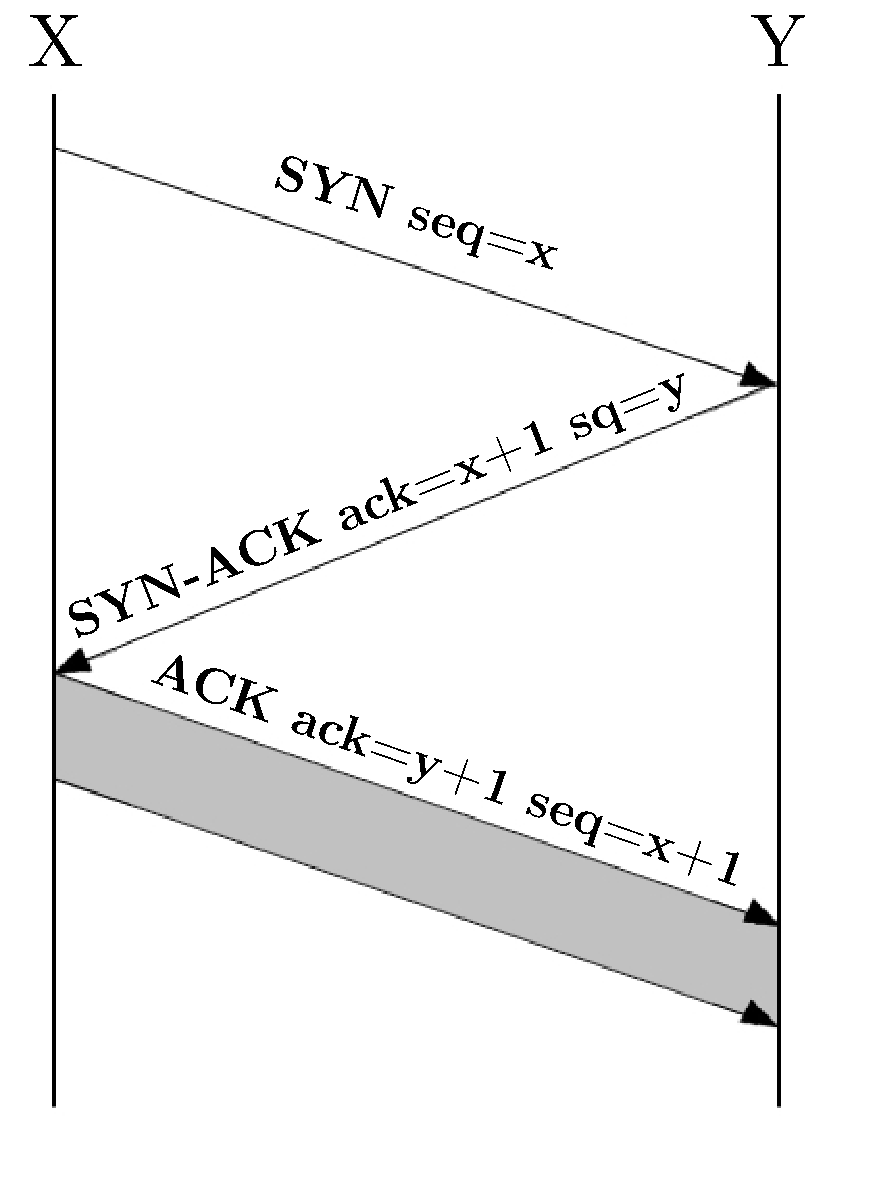
\includegraphics[width=0.5\textwidth]{./images/TCPHandshake.pdf}%
		\label{fig:TCPHandshake}%
	}%
	\hfill
	\subfigure[SYN Flooding]{%
		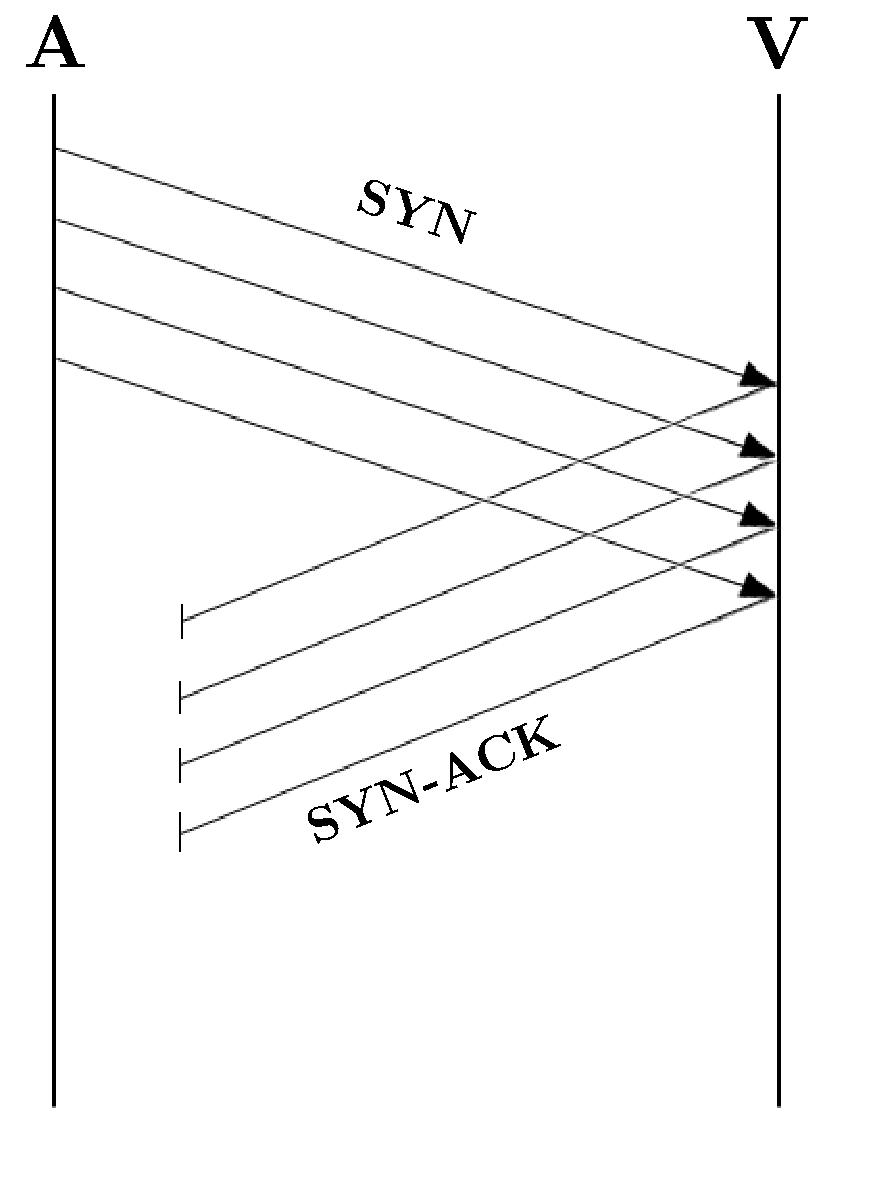
\includegraphics[width=0.5\textwidth]{./images/TCPSynAttak.pdf}%
		\label{fig:SYNFlooding}%
	}%
	\caption{TCP Tree-way handshake and SYN Flooding} 
	\label{fig:TCPConnections}
\end{figure}


\subsection{Methods of Attacks}

The attack can be categorized depending on how the attacker carries out the attack over the victim: Direct Attack, Spoofed-based Attack and Distributed Attack ~\cite{CiscoTCPSYN}.

\subsubsection{Direct Attack}

\subsubsection{Sppofed-based Attack}

\subsubsection{Distributed Attack}

\subsection{Prevention and Response}



\subsection{Tercer apartado}

